\chapter{Motor Driver}
\label{chap:Motor_Driver}
%------------------------------------------------

\par As the name suggests, motor drivers are used to drive the motors. Motors consume higher current, more that what Arduino can supply. Hence they are interfaced with Arduino board using a motor driver. The motor driver consumes the power from external source and direct them to motors, controlled by Arduino. There are various motor drivers available. You might also able to find Arduino shields for motor drivers. A motor driver shield is much more powerful motor driver that can handle various DC motors, stepper motors, servo motors. In this session we would be talking about a simple motor driver - L298N

\begin{marginfigure}
\centering
  % include first image
  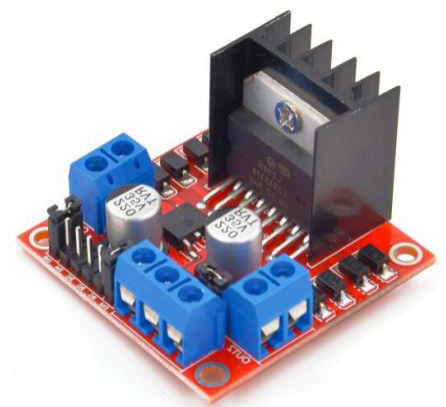
\includegraphics[width=.8\linewidth]{Chapters/images/MotorDriver_board.png}  
  \caption{Put your sub-caption here}
  
\end{marginfigure}

\begin{marginfigure}
\centering
  % include first image
  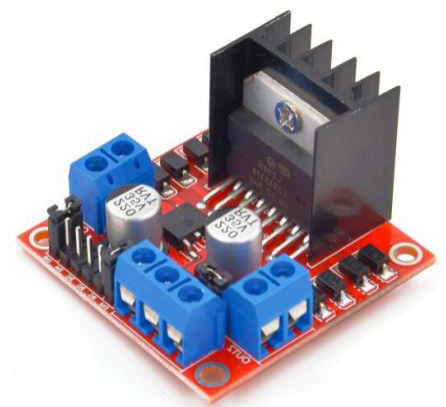
\includegraphics[width=.8\linewidth]{Chapters/images/MotorDriver_board.png}  
  \caption{Put your sub-caption here}
  
\end{marginfigure}
\section{L289N motor driver}
L298N motor driver is one of the many motor drivers available in the market. This driver have 4 out lines grouped into two as channel A and channel B. The working of the board is simple. Connect the external power source ( ~12V) to the +12V pin and the negative terminal of the source to the GND pin. Since we need to interface it with Arduino, we need connect the GND pin of Arduino to the GND pin of the board. The logical signals are supplied from Arduino to the board on the pins input1 to input4. When any of the logical pins are high, corresponding OUT pin turns on and gives an output of 10V. For example, if input3 is turned to HIGH, OUT3 would provide 10V and if input 2 is LOW, OUT2 would be at zero volt. \\
\begin{figure}
    \centering
    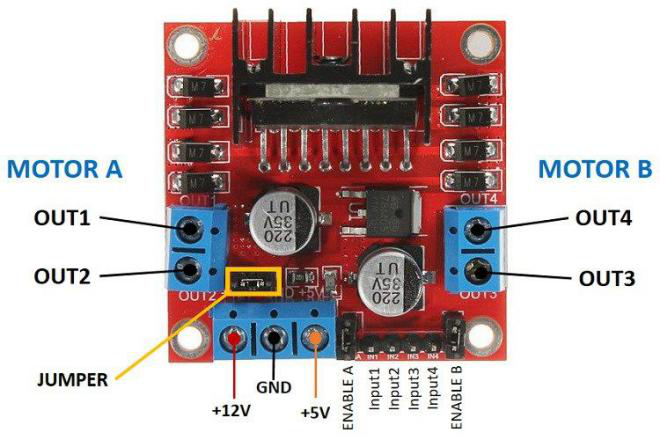
\includegraphics[width=2in]{Chapters/images/MotorDriver_desp.png}
    \caption{MotorDriver Description}
    \setfloatalignment{b}
\end{figure}
We can also find three jumper settings on the board. The jumper just above the power source (12V) connects the 5V pin via 5V regulator. The 5V pin is used to power IC on board. If the external power source is about 10 to 12 volts, we can keep this jumper on to power the board and motors using the 12V input. At this time, the 5V pin can act as an 5V output pin and can be used to power up the Arduino board. If we are providing external power supply greater than 12V, remove the jumper settings. The 5V regulator can get damaged. At this time, we would require additional 5V supply from Arduino to power the IC. L298N can handle up-to 35volts of external supply. Keep in mind that the board draws higher current and can exhaust your battery. Providing higher voltages can also cause the IC’s to heat up rapidly. Make sure to cool them if they crosses the threshold. \\
The second jumper you can find are at either sides of the logical input pins. On the left side we have jumper for channel A and on right side for channel B. These pins actually control the speed of the motors. To adjust the speed of motor in each channel, remove the jumpers and connect PWM pins of Arduino to control the speeds. If you want to function the motors at full capacity, keep the jumper ON.

\section{Interfacing DC motor - motor driver - Arduino}
\label{section:bot_interface}

Let us connect the motor driver and Arduino. The driver would be powered up via external supply and Arduino will be powered via USB cable. In this sample connection, lets connect and 10V DC motor to each channels. The next question is, how to control the direction of the motors? Lets consider the channel A. The terminal of the motor is connected to the OUT pins.
\begin{figure}
    \centering
    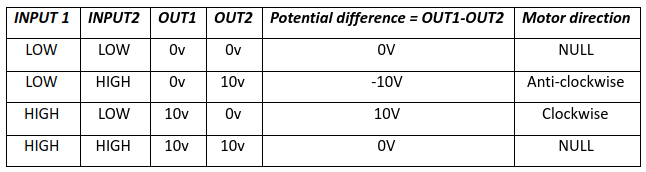
\includegraphics{Chapters/images/md1.png}
\end{figure}
\\ From the table below, it is clear that by inverting the logical signals, we can change the direction of motor. The same can be applied at the channel B for direction control. Now lets make the connections!

\begin{figure}
    \centering
    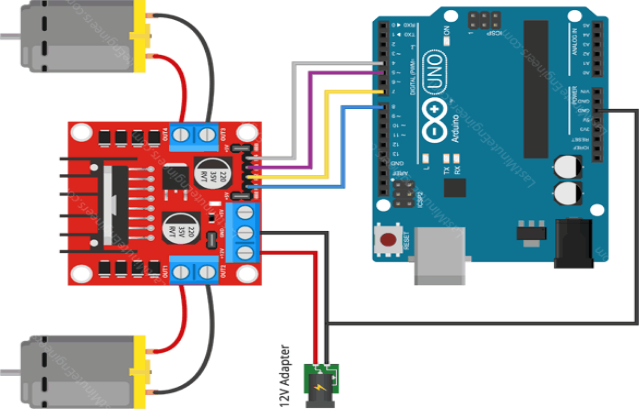
\includegraphics[width=2in]{Chapters/images/MotorDriver_circuit1.png}
    \caption{Interfacing MotorDriver with Arduino}
    \setfloatalignment{b}
\end{figure}

As shown in the figure, we have connected pins 8, 7, 5, 4 to input1, input2, input3 and input4 respectively. Both the boards shares the common GND and the driver is powered via 12V supply. Let’s write a program that turns the motors clockwise and anti clockwise to control the bot movement.\\

Code\\
\begin{lstlisting}[style=CStyle]
int m1 = 8, m2 = 7;  //left  motor pins
int m3 = 5, m4 = 4;  //right motor pins

void setup(){
//set motor pins as output for Arduino.
pinMode(m1,OUTPUT); pinMode(m2,OUTPUT);
pinMode(m3,OUTPUT); pinMode(m4,OUTPUT);
Serial.begin(9600);
}

//A function to control motor movement
void turn_motor(int input1, int input2, char dir){
if( dir == 'F'){
//clockwise rotation
digitalWrite(input1,HIGH);
digitalWrite(input2,LOW);
}
else if( dir == 'B'){
//anti-clockwise rotation
digitalWrite(input1,LOW);
digitalWrite(input2,HIGH);
}
else if( dir == 'S'){
//no rotation
digitalWrite(input1,LOW);
digitalWrite(input2,LOW);
}
}

void loop(){

turn_motor(m1, m2, 'F');  //left  wheel : clockwise
turn_motor(m3, m4, 'F');  //right wheel : clockwise
Serial.println("Bot moving forward");
delay(1000);

turn_motor(m1, m2, 'B');  //left  wheel : anti-clockwise
turn_motor(m3, m4, 'F');  //right wheel : clockwise
Serial.println("Bot turning left (rapidly)");
delay(500);

turn_motor(m1, m2, 'F');  //left  wheel : clockwise
turn_motor(m3, m4, 'B');  //right wheel : anti-clockwise
Serial.println("Bot turning right (rapidly)");
delay(500);

turn_motor(m1, m2, 'B');  //left  wheel : anti-clockwise
turn_motor(m3, m4, 'B');  //right wheel : anti-clockwise
Serial.println("Bot moving backward");
delay(1000);

turn_motor(m1, m2, 'S');  //left  wheel : stop
turn_motor(m3, m4, 'S');  //right wheel : stop
Serial.println("Bot stopped");
delay(5000);
}

\end{lstlisting}

Let’s summarize the bot movement of the above program.\\
\begin{figure}
    \centering
    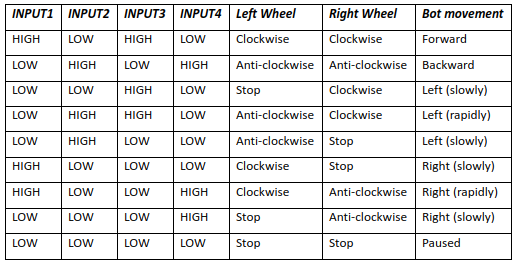
\includegraphics{Chapters/images/md2.png}
\end{figure} \\
You might have noticed that the bot drifts or becomes unstable when it changes it direction suddenly. This is because the wheels are rotating with higher speed than our bot can handle. The solution to such problems is the control the speed of the wheels. This can be easily achieved by making use of PWM pins in the motor driver. Lets try out our new speed controlled bot. It is easy to modify the above circuit and code to build the new bot quickly.

\section{Speed controlled Bot}
Re-configure the circuit by removing the jumper pins of channel A and B. Connect PWM pins 9 and 3 of Arduino to channel A and channel B respectively. You can identify PWM pins in Arduino by noticing the tilde symbol ( ~ ) on the board. The new circuit might look like this.
\begin{figure}
    \centering
    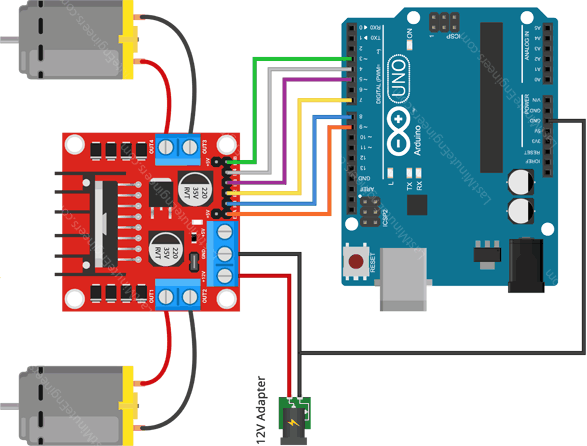
\includegraphics[width=2in]{Chapters/images/MotorDriver_circuit2.png}
    \caption{Interfacing Motors}
    \setfloatalignment{b}
\end{figure} \\
Now lets reconfigure the program \\
Code\\
\begin{lstlisting}[style=CStyle]
int pwmL = 9, m1 = 8, m2 = 7;  //left  motor pins
int pwmR = 3, m3 = 5, m4 = 4;  //right motor pins

void setup(){
//set motor pins as output for Arduino.
pinMode(m1,OUTPUT); pinMode(m2,OUTPUT); pinMode(pwmL,OUTPUT);
pinMode(m3,OUTPUT); pinMode(m4,OUTPUT); pinMode(pwmR,OUTPUT);
Serial.begin(9600);
}

//A function to control motor movement with speed regulation
void turn_motor(int input1, int input2, int speed_pin, int speed, char dir){
//Setting the speed
analogWrite(speed_pin, speed);

if( dir == 'F'){			//clockwise rotation
digitalWrite(input1,HIGH);
digitalWrite(input2,LOW);
}
else if( dir == 'B'){	//anti-clockwise rotation
digitalWrite(input1,LOW);
digitalWrite(input2,HIGH);
}
else if( dir == 'S'){	//no rotation
digitalWrite(input1,LOW);
digitalWrite(input2,LOW);
}
}

void loop(){

turn_motor(m1, m2, pwmL, 255, 'F');  //left  wheel : clockwise, speed=100%
turn_motor(m3, m4, pwmR, 127, 'F');  //right wheel : clockwise, speed=50%
Serial.println("Bot moving forward with small right curve");
delay(1000);

turn_motor(m1, m2, pwmL, 0, 'F');    //left  wheel : clockwise, speed=0%
turn_motor(m3, m4, pwmR, 127, 'F');  //right wheel : clockwise, speed=50%
Serial.println("Bot moving left with low speed");
delay(1000);
}

\end{lstlisting}
Keep in mind that PWM pins are 8-bit support pins. The Maximum analog value we can send is 255 i.e., $ 2^8 - 1 $ [ counting starts from zero ]. If PWM value is set to 255, the motors will run at full capacity and would decrease as the value decreases. Do note that you are controlling the effective voltage sent to the motor and not the actual wheel rotation. To control the rotation of the wheel precisely, we would have to make use of stepper motors.
\begin{figure}
    \centering
    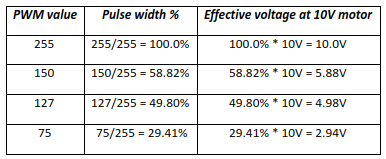
\includegraphics{Chapters/images/md3.png}
\end{figure}
Try connecting few sensors like Ultrasonic sensors, IR sensor, LDR, Accelerometer etc to make your bot autonomous and attractive!
\begin{figure}
    \centering
    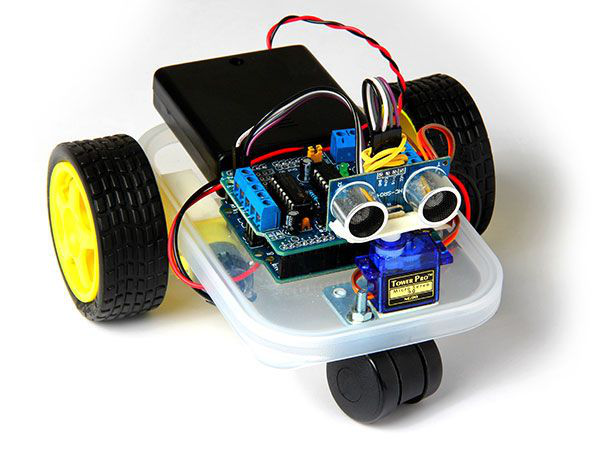
\includegraphics[width=3.2in]{Chapters/images/MotorDriver_end_pic.png}
    \caption{A Bot}
    \setfloatalignment{b}
\end{figure}